\documentclass[12pt]{article}
\usepackage{amsmath}
\usepackage{amssymb}
\usepackage{amsfonts}
\usepackage[polish]{babel}
\usepackage[T1]{fontenc}
\usepackage[dvips]{graphicx}
\usepackage[cp1250]{inputenc}
\usepackage{listings}
\usepackage{pdfpages}
\usepackage{float}

\restylefloat{table}

\textheight 23.2 cm

\textwidth 6.0 in

\hoffset = -0.5 in

\voffset = -2.4 cm

\hyphenation{}

\frenchspacing

\begin{document}

\vspace*{3ex}
\begin{flushright}
{\large 26 May 2019}
\end{flushright}

\begin{flushleft}
{\large Patryk \.Walczak\\
Group 2}
\end{flushleft}

\hskip3cm

\begin{center}

{\large Project 10}

\Large {\bf Finding a root of the complex polynomial p(x) using the King method and Horner scheme, where}
\begin{equation*}
p(x) = \sum_{k=0}^n a_{k} x^{k}.
\end{equation*}
\end{center}

\vskip2ex



\pagebreak

\begin{center}
\item \section{Method description}
\end{center}

\bigskip The King method is iterative method of finding root of the funciotn $f(x)$, more precisely in the task finding root of polynomial $p(x)$. Constructing  a sequence ${x_{k}}$ such that $x_{k} \approx \alpha$, where $f(\alpha) = 0$, using formulas:

\begin{equation*}
y_{k}=x_{k} - \frac{f(x_{k})}{f'(x_{k})}
\end{equation*}

\begin{equation*}
x_{k+1}=y_{k} - \frac{f(y_{k})}{f'(y_{k)}} -\frac{f(x_{k})}{f'(x_{k})} \Bigg( \frac{f(y_{k})}{f(x_{k})} \Bigg) ^3
\end{equation*}

\vskip20pt

Starting from a given initial guess $x_{0}$ we construct a sequence ${x_{k}}$ of approximations, such that $ x_{k} \rightarrow \alpha$ as $k \rightarrow \infty $.

\vskip20pt

Horner sheme is method of evalution polynomial value for received data. This sheme allows evaluation of a polynomial of degree n with only n multiplications and n additions. This is optimal, since there are polynomials of degree n that cannot be evaluated with fewer arithmetic operations. Horner's method formula for polynimials looks like 

\begin{equation*}
p(x)=a_{0}+a_{1}x+a_{2}x^{2}+a_{3}x^{3}+ \cdots +a_{n}x^{n}= a_{0}+x{\bigg (}a_{1}+x{\Big (}a_{2}+x{\big (}a_{3}+\cdots +x(a_{n-1}+x\,a_{n})\cdots {\big )}{\Big )}{\bigg )}.
\end{equation*}

In the project, Horner scheme is used for every evaluation of polynomial value and value of polynomial derivative in the King method.

\pagebreak

\begin{center}
\item \section{Description of Matlab program}
\end{center}

\noindent After run the program, the Menu appears:

\vskip3ex
\begin{center}
\hspace*{-2ex}
\begin{tabular}{|c|} \hline
\\
{\bf Menu}
\\\\Change the complex polynomial
\\\\Change initial x0
\\\\Change error tolerance
\\\\Change number of maximal iterations
\\\\Change interval of plot
\\\\Change example
\\\\Display variables
\\\\Compute root of the polynomial
\\\\FINISH
\\\\
\hline
\end{tabular}
\end{center}

\vskip3ex
After pushing:
\begin{itemize}
\item Change the complex polynomial - user will be able to input their own roots of polynomial. The program compute coefficients of polynomial using matlab function 'poly([set of user's roots])', that is the easer way to input polynomial, but that is also possibility to input coefficients of polynomial.
\item Change initial x0 - user will be able to input their own initial value of $x_{0}$.
\item Change error tolerance - user will be able to input their own tolerance of error.
\item Change number of maximal iterations - user will be able to input their own limit of iterations.
\item Change example - change the default variables.
\item Display variables -  user will be able to see all variables.
\item Compute root of the polynomial - program computes root of polynomial using the King Method and Horner scheme, then prints score on screen and value of the polynomial of the root to be sure that score is correct.
\item FINISH - program will finish.
\end{itemize}

\bigskip

\noindent MATLAB functions:
\begin{enumerate}
\item Menu.m - script for graphic interface of menu, which uses rest of functions.
\item King.m - function strictly for computing root of polynomial with the King method, using initial $x_{0}$ iterate to obtain root (with $\pm$ error), or obtain maximal amount of iterations, then return root and number of iteration
\item Horner.m - fuction evaluates value of polynomial for input polynomial and value of x .

\noindent ({\bf Note.} \emph{All source codes can be found in section 5.})
\end{enumerate}

\vskip20pt

\begin{center}
\section{Numerical tests}
\end{center}

\vskip20pt

\noindent
All the numerical tests are included in the Menu.m file, while user pushes button 'Change example', the example data are changed. Program computes the value of root (if it obtains before number of maximal iteration), and return amount of iterations. Then plot of real value of the polynomial appears.
In every test the variables are different, for checking the correctnes of program there is error also.

\bigskip

\textbf{Tests:}

Polynomial is obtained by input roots and evaluate coefficents by matlab function "poly([set of roots])".
In every example is choosed initial value of $ x_{0}$ from that program will start compute root.

\begin{enumerate}

\vskip20pt

\item
Initial roots are $a=[1,-2,5]$ from the set obtained polynomial is\\
\begin{equation*}
p(x)=1x^3  -4x^2    -7x    +10,
\end{equation*}
where initial value of $x_{0}$ is equal 3.
The tolerance error is equal $1e^{-10}$ \\and number of maximal iteration is equal 100.
\\Moreover interval of plot is $[-2.5,5.5]$ to see all roots. 

\vskip20pt

Program returns:
\begin{center}
King method after 1 iterations returns value root = -2\\
and value of the polynomial for root = 0
\end{center}

\begin{center}
   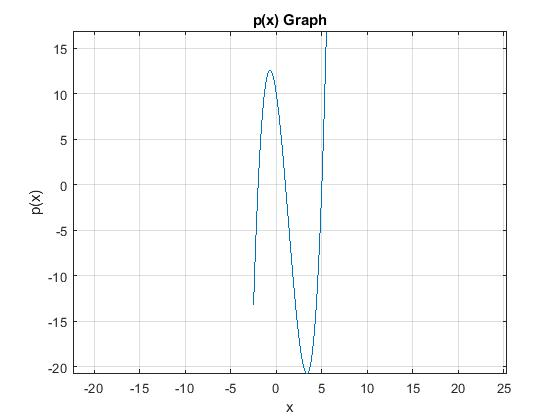
\includegraphics[scale=0.6]{Example_1.jpg}
\end{center}

From graph is known that program computes root correctly.

\vskip50pt

\item

Initial roots are $a=ones(1,6)$ from the set obtained polynomial is\\
\begin{equation*}
p(x)=1x^6    -6x^5    +15x^4   -20x^3    +15x^2    -6x     +1,
\end{equation*}
where initial value of $x_{0}$ is equal 3.
The tolerance error is equal $1e^{-10}$ \\and number of maximal iteration is equal 100.
\\Moreover interval of plot is $[0,2]$ to see all roots. 

\vskip20pt

Program returns:
\begin{center}
King method after 13 iterations returns value root = 1.015531e+00\\
and value of the polynomial for root = 1.403233e-11
\end{center}

\begin{center}
   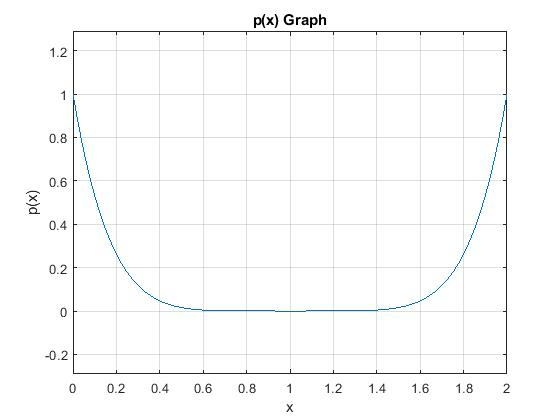
\includegraphics[scale=0.6]{Example_2.jpg}
\end{center}

From graph is known that program compute root correctly. Value of the polynomial is close to 0 ($1.403233e^{-11} = 0.00000000001403233$) and thats is less then error.


\vskip50pt

\item

In the example, roots are random, and they are complex numbers to check correctners of the program for comples numbers. 
Initial roots are $a=randn(1)+2i$ from the set obtained polynomial is\\
\begin{equation*}p(x)= 
p(x)=   (1.0000 + 0.0000i)x  -0.8622 - 2.0000i
\end{equation*}
where initial value of $x_{0}$ is equal -1.
The tolerance error is equal $1e^{-10}$ \\and number of maximal iteration is equal 100.
\\Moreover interval of plot is $[-2,2]$ to see all roots. 

\vskip20pt

Program returns:
\begin{center}
King method after 1 iterations returns value root = 8.621733e-01\\
and value of the polynomial for root = 0
\end{center}

\begin{center}
   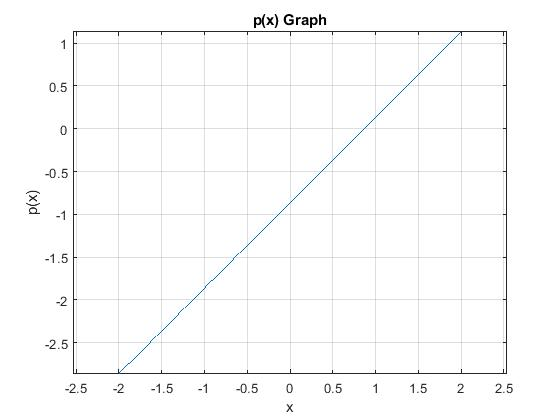
\includegraphics[scale=0.6]{Example_3.jpg}
\end{center}

From graph is known that program computes root correctly even for complex numbers. But because graph is for real numbers there is no imaginaru part of polynomial value.

\item             

This is the example with the error, to be sure that program can not compute root for bad choosed number.
Initial roots are $a=[1:25]$ from the set obtained polynomial is

\begin{multline*}
p(x)=
   -0.0003    x^{10}  +0.0020   x^9  -0.0100    x^8  +0.0414   x^7  -0.1375
    x^6 \\ +0.3577   x^5  -0.7087  x^4  +1.0234   x^3  -1.0048    x^2  +0.5919  x  -0.1551
\end{multline*}

where initial value of $x_{0}$ is equal 1000.
The tolerance error is equal $1e^{-10}$ \\and number of maximal iteration is equal 100.
\\Moreover interval of plot is $[0,25]$ to see all roots. 

\end{enumerate}

\vskip20pt

Program return:
\begin{center}
King method after 101 iterations return value root = -1.339470e+07
and value of the polynomial for root = -1.490524e+178
\end{center}

\begin{center}
   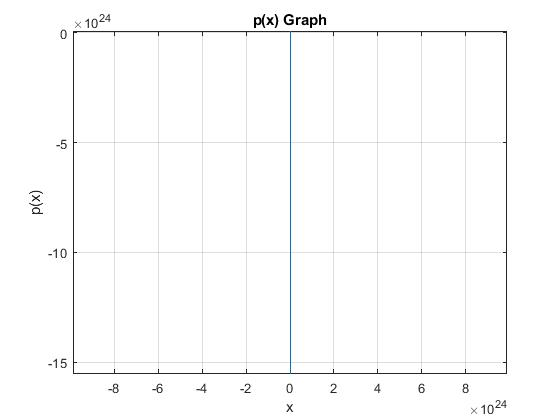
\includegraphics[scale=0.6]{Example_4.jpg}
\end{center}

Here program obtains 100 iterations and returns no correct root. For too big initial value of $x_{0}$ 100 iteration is too small amount of iterations.

\begin{center}
\section{Conclusion}
\end{center}

\begin{flushleft}
First what is mentioned in the raport Horner scheme is efficient way of computing value of polynomial. Secondly, the succes of the finding root of polynomial using the King method is dependent of the initial value of $x_{0}$. Both algorithms works for complex numbers what is proved above. Moreover the King method coincides fast to the value of the root. Although it computes value of root with really low amount of iterations,that always finds only one root, what is usefull if we search any root, but that is no such usefull when we need all roots.
\end{flushleft}

\begin{center}
\item \section{Source Codes}
\end{center}

{\bf Is\_Hessenberg.m :}
\lstinputlisting{King.m}

\pagebreak

{\bf Jacobi\_Method.m :}
\lstinputlisting{Horner.m}

\pagebreak

{\bf Menu.m:}
\lstinputlisting{Menu.m}

\end{document}
